  \documentclass[twoside=false, %  doppelseitiger Druck
    DIV=15,% DIV Faktor für Satzspiegelberechnung, sie Doku zu KOMA Script
    BCOR=15mm, % Bindekorrektur
    chapterprefix=false,
    headinclude=true,
    footinclude=false,
    pagesize,%         write pagesize to DVI or PDF
    fontsize=12pt,%             use this font size
    paper=a4,%          use ISO A4         write bibliography-chapter to table of contents
    index=totoc,%         write index-chapter to table of contents
    cleardoublepage=plain,% \cleardoublepage generates pages with pagestyle empty
     headings=big,%       A4/B5
    listof=flat,%        improved list of tables
    numbers=noenddot
  ]{scrbook}
\usepackage{listings}
\usepackage{url}
\usepackage[utf8]{inputenc}
\usepackage{makeidx}
\usepackage{amsfonts}
\usepackage[slantedGreek,sc]{mathpazo}  % Schriftart Palatino
% \usepackage{lmodern}    % statt mathpazo, falls CM Fonts verwendet werden sollen
%\usepackage{mathptmx}    % statt mathpazo, falls Times  verwendet werden soll
\usepackage[scaled=.95]{helvet}
\usepackage{courier}
\usepackage[T1]{fontenc}
\usepackage{textcomp}
\usepackage{amsmath}            % standard math notation (vectors/sets/...)
\usepackage{bm}        % standard math notation (fonts)
\usepackage{fixmath}        % standard math notation (fonts)
\usepackage{graphicx}
\usepackage[facing=yes]{floatrow}       % mehrere Gleitobjekte nebeneinander/caption neben Bild/Tabelle
\usepackage[labelfont=bf,sf,font=small,labelsep=space,format=plain]{caption}
\usepackage{subcaption}
\usepackage{scrlayer-scrpage}
% \usepackage{pstool}  % einbinden falls psfrag verwendet werden soll
\usepackage{epstopdf}
\usepackage[ngerman]{babel}
\usepackage{ellipsis}  % Korrigiert den Weißraum um Auslassungspunkte
\usepackage{microtype}  % optischer Randausgleich etc.

\usepackage{xcolor}         % z.B. für schattierte Boxen
\usepackage{framed}			% shaded Umgebung
\definecolor{shadecolor}{gray}{.85}%

% Links im PDF
\usepackage[colorlinks=false,
            pdfborder={0 0 0},
            breaklinks=true]
            {hyperref}


%\typearea[current]{calc}


% Einstellungen für Bild-/Tabellenbeschriftung neben dem Bild
\floatsetup[figure]{capbesideposition={inside,top}}
\floatsetup[table]{capbesideposition={inside,top},style=plaintop}
\renewfloatcommand{fcapside}{figure}[\capbeside][\FBwidth]
\newfloatcommand{tcapside}{table}[\capbeside][\FBwidth]

\lstset{
	language=java,
	basicstyle=\ttfamily
}

\selectlanguage{ngerman}


\deffootnote{1em}{1em}{%
 \makebox[1em][l]{\thefootnotemark}}

\makeindex

\newcommand{\real}{\mathord{\mathrm{I\!R}}}

\begin{document}
\selectlanguage{ngerman}
\def\figdir{figures}
\def\tabledir{tables}

\frontmatter

\pagestyle{scrplain}
\pagestyle{empty}

\begin{titlepage}

\sffamily

\raggedleft

\vspace*{-2cm}


\includegraphics{\figdir/logo-th-rosenheim-2019_master_quer_2c.eps}

\vfill

\centering
\LARGE
% \vspace*{\fill}
%-----------
Fakultät für Informatik  \vspace{0.5cm}\\
\Large
FWPM Penetrationstests und Forensik


\vspace{2cm}

\LARGE

Abschlussbericht Forensik

\vspace{2cm}

\Large


\vspace{1.5cm}


\Large
von

\vspace{0.5cm}

%\vspace*{\fill}

\LARGE
Daniel Böning \vspace{1cm} \\
Jonathan Hamberger \vspace{1cm} \\
Osman Güloglu \vspace{1cm} \\
Karl Herzog \vspace{1cm} \\

\vspace{1cm}

\flushleft
 \Large
\vspace*{\fill}

\end{titlepage}

\cleardoubleemptypage

%%% Local Variables: 
%%% mode: latex
%%% TeX-master: "d"
%%% End: 

\cleardoubleemptypage

\pagestyle{scrplain}
\pagenumbering{roman}
% ---------------------------------------------------
% D-TOC.TEX zur Verwendung mit TEXPART
% (an eigene Gegebenheiten anzupassen)
% ---------------------------------------------------
%
\tableofcontents


\pagestyle{scrheadings}


\addtokomafont{caption}{\small}

\mainmatter

\chapter{Analyse des kompromittierten Systems}

\section{Einleitung}
Beim  Reiseveranstalter „hVs-Reisen“, der auf Reisen nach Nordkorea spezialisiert ist, kam es am Nachmittag des 14.11.2017 zu einem Security Incident, nachdem der

Virenscanner auf dem virtuellen Client des Mitarbeiters Lars Walter eine Malware

erkannt hatte.

Das Forensik Team wurde daraufhin beauftragt, das betroffene System einer forensischen Analyse zu unterziehen. Der vorliegende Bericht gliedert sich in eine sog. Management Summary, in welcher die wichtigsten Ergebnisse der Untersuchung in kompakter Form dargestellt sind. Im Anschluss daran folgt eine detaillierte Aufstellung der Vorgehensweise und Ergebnisse, in der speziell auf die Fragen des Kunden eingegangen wird. Abgeschlossen wird der Bericht mit Handlungsempfehlungen für den Kunden von Seiten des Forensik Teams.

\chapter{Analyse des Systems}

\section{Vorbereitung}
Zur Durchführung der forensischen Analyse wurden dem Team zwei Sicherungsdateien des betroffenen Clients des Mitarbeiters Lars Walter zur Verfügung gestellt. Dabei handelt es sich zum Einen um die Sicherung des Arbeitsspeichers \textit{client-walter.vmem} und zum Anderen um ein Image der Festplatte (client-walter.vmem). 
Zu Beginn wurde die Integrität der Images überprüft. Dabei wurden vom Team die Hashwerte der beiden Dateien mit dem CertUtil Befehl ermittelt und mit den vom Kunden zur Verfügung gestellten Hashwerten verglichen.


\begin{center}
	\begin{tabular}{|c|c|c|c|c|} 
		\hline
		Datei & Sicherungszeitpunkt & MD5 & SHA1 & SHA256 \\ [0.5ex] 
		\hline
		client-walter.vmem & 14.11.17 16:00 Uhr & korrekt & korrekt & korrekt \\ 
		\hline
		client-walter.e01 & 27.11.17 14:00 Uhr & korrekt & korrekt & korrekt \\ 
		\hline
	\end{tabular}
\end{center}

Da eine Übereinstimmung der Hashwerte festgestellt wurde, konnte davon ausgegangen werden, dass die Daten korrekt übermittelt wurden. Sie konnten daher zur weiteren forensischen Analyse herangezogen werden.

\section{File Records in Master File Table (MFT)}
Die MFT-Datei des betroffenen Clients wurde mithilfe von FTK Imager extrahiert und anschließend mithilfe von Mft2csv in eine CSV-Datei umgewandelt. 
Als Ergebnis lässt sich Folgendes festhalten: Im Cache für Email-Anhänge konnte die Existenz einer .zip- Datei \path{Temp1_171110_NorthKorea-DiploimaticUpdate.zip} nachgewiesen werden, in der die eigentliche Malware enthalten war. \path{171110_NorthKorea-DiploimaticUpdate.pdf.exe} Darüber hinaus konnte eine entsprechende Prefetch-Datei \path{171110_NORTHKOREA-DIPLOIMATIC-3B19E785.pf} nachgewiesen werden. Dies ist in Abbildung \ref{fig:mft} ersichtlich.

\begin{center}
	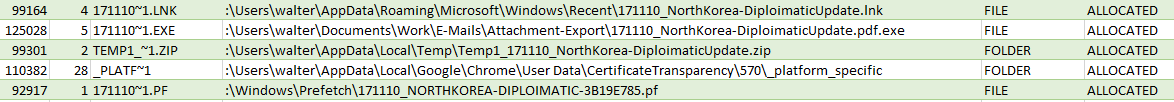
\includegraphics[width=15.8cm]{figures/mft.png}
	\captionof{figure}{MFT }
	\label{fig:mft}
\end{center}

\section{Prefetch-Files}
Mithilfe des Tools PECmd wurde das zur Malware gehörende Prefetch-File \path{/Windows/Prefetch/171110_NORTHKOREA-DIPLOIMATIC-3B19E785.pf} analysiert. Das Ergebnis ist in Abbildung \ref{fig:prefetch}
Es konnte nachgewiesen werden, dass die Malware zuletzt am 13.11.17 um 16:27 Uhr ausgeführt wurde. Dies lässt den Schluss zu, dass der Client des Mitarbeiters schon einen Tag vor dem Security Incident am 14.11.17 kompromittiert war.

\begin{center}
	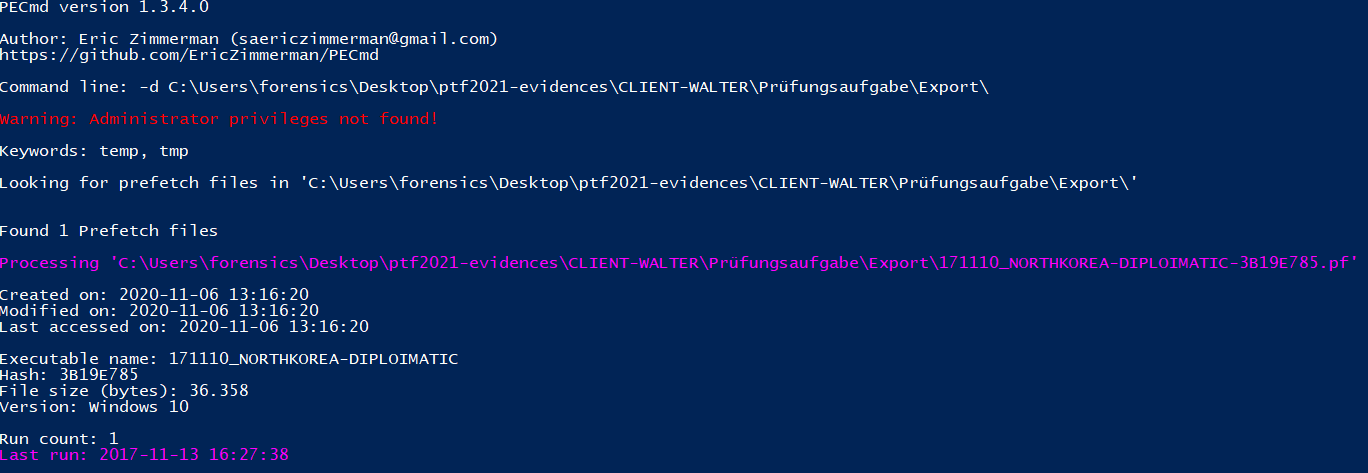
\includegraphics[width=15.8cm]{figures/prefetch.png}
	\captionof{figure}{MFT }
	\label{fig:prefetch}
\end{center}

\section{Registry-Analyse}
Es wurde eine Analyse der Registry Dateien NTUSER.dat, SYSTEM.dat, SAM.dat, SECURITY.dat und SOFTWARE.dat durchgeführt. Diese Dateien wurden aus dem Dateisystem des kompromittierten Rechners extrahiert und mit dem Programm RegRipper analysiert.

Die NTUSER Datei enthielt folgenden Eintrag unter dem Abschnitt UserAssist:
\\
\begin{center}
	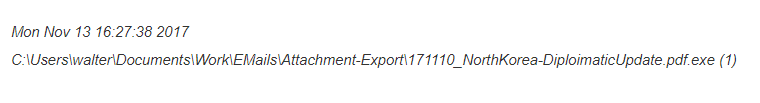
\includegraphics[width=15.8cm]{figures/prefetch_path.png}
	\captionof{figure}{Pfad zur verdächtigen Datei}
	\label{fig:prefetch_path}
\end{center}

Diese Datei konnte aus dem Dateisystem des betroffenen Rechners extrahiert werden und wurde mit VirusTotal analysiert. In Abbildung \ref{fig:vtprefetch}  sind die Ergebnisse von VirusTotal zu sehen.

\begin{center}
	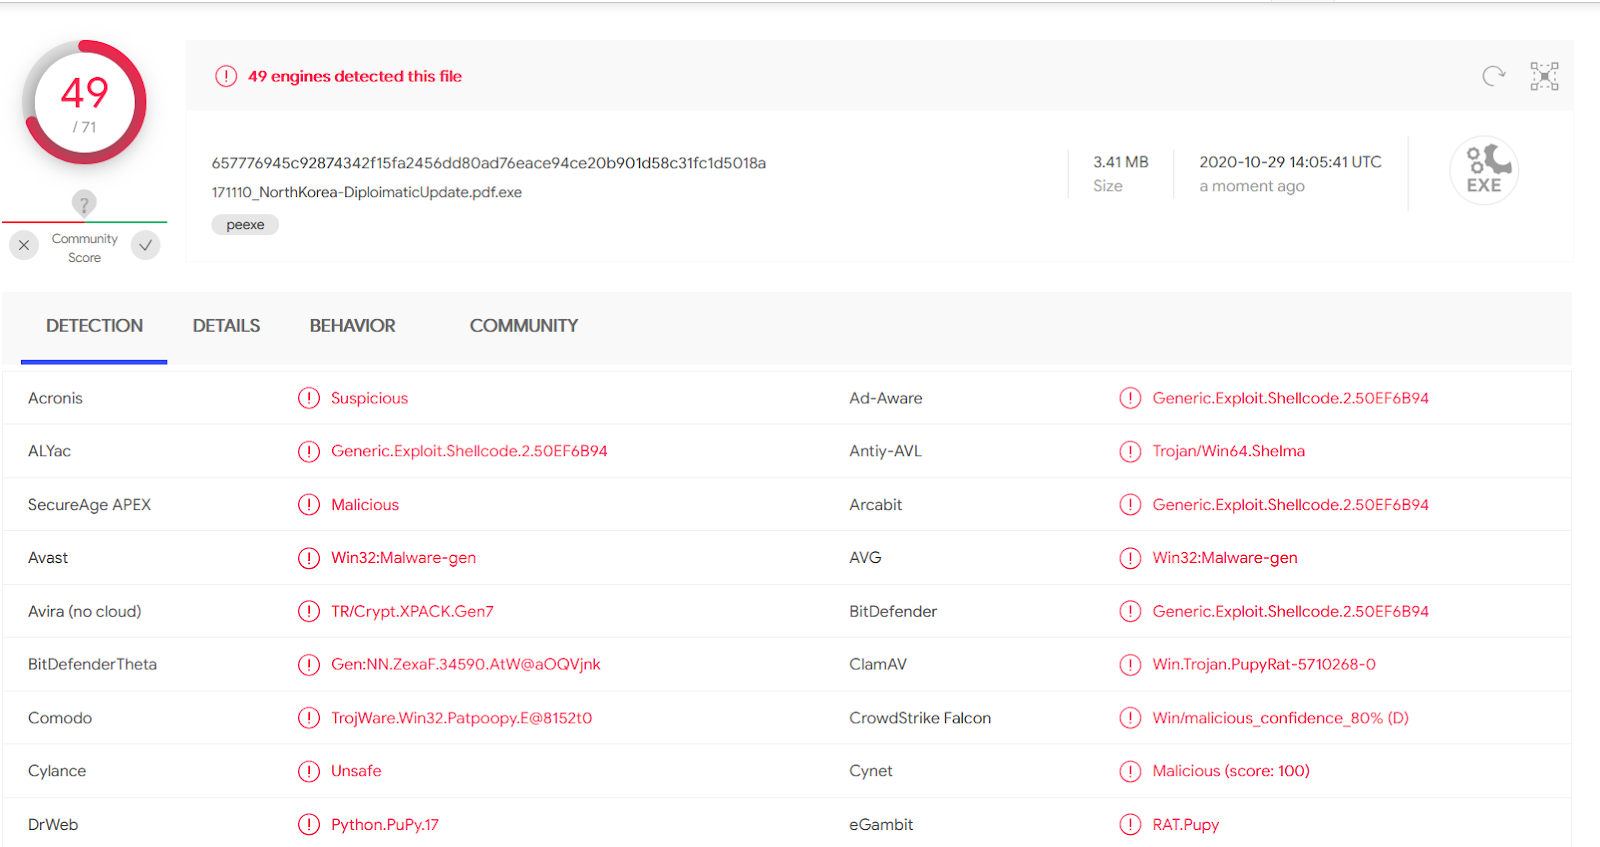
\includegraphics[width=15.8cm]{figures/virustotal_prefetch.png}
	\captionof{figure}{VirusTotal der prefetch Datei}
	\label{fig:vtprefetch}
\end{center}

Zusätzlich wurde in der\textit{ NTUSER.dat} Datei der Key RecentDocs analysiert. Es stellte sich dabei heraus, dass diese Datei zum letzten am am 01.01.1970 um 00:00 Uhr geschrieben wurde. Es ist zu vermuten, dass der Angreifer den Attribut LastWrite auf Beginn der Unixzeit \textit{1. Januar 1970, 00:00 Uhr} bewusst gesetzt hat und somit eine Manipulation zur Verschleierung von Spuren hindeuten könnte.

Ein Ausschnitt aus der RecentDocs-Analyse ist in Abbildung \ref{} zu sehen.
\begin{center}
	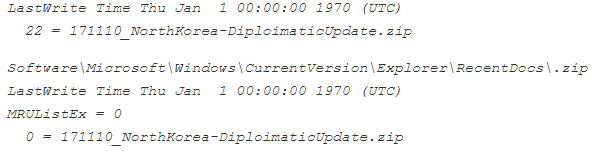
\includegraphics[width=15.8cm]{figures/prefetch_manipulation.png}
	\captionof{figure}{Ausschnitt aus der RecentDocs-Analyse}
	\label{fig:prefetch_manipulation}
\end{center}

Die SECURITY.dat und SAM.dat Dateien enthielten keine aufschlussreichen Einträge.


Um den letzten Login im System festzustellen, wurde die Datei \textit{SOFTWARE.dat} analysiert. Dabei stellte sich ebenfalls raus, dass der Eintrag Winlogon überschrieben wurde. Auch hier ist davon auszugehen, dass der Angreifer diesen Eintrag überschrieben hat, um seine Spuren zu verwischen. Der zuletzt eingeloggte User sowie der Zeitpunkt des Logins konnten somit nicht ermittelt werden. Dies ist in Abbildung \ref{fig:softwaredat} zu sehen.

\begin{center}
	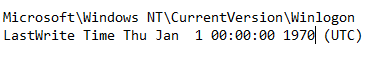
\includegraphics[width=15.8cm]{figures/softwaredat.png}
	\captionof{figure}{Ein Ausschnitt aus der Software.dat Analyse}
	\label{fig:softwaredat}
\end{center}

Die Ermittlungen ergaben, dass neben den bereits erwähnten Manipulationen, weitere Zugriffszeiten in allen Registry-Einträgen zurückgesetzt wurden.

\section{Wireshark Analyse}
Wireshark wurde am 13.11.17 um 16:24 Uhr herunterladen und eine Minute vor der eigentlichen Malware um 16:26 Uhr gestartet. Es deutet darauf hin, dass der Mitarbeiter aufgrund eines ersten Verdachts das Sniffing-Tool selbst heruntergeladen hat, um den Netzwerkverkehr von seinem Rechner zu überwachen. Außerdem wurde eine Wireshark-Erweiterung \textbf{Solarwinds Response Time Viewer} installiert. Dies ist in Abbildung \ref{fig:wireshark_history} und \ref{fig:wireshark_paths} zu sehen. Im Image des Users findet sicher unter \path{/root/Install} zwei Wireshark Dumps \path{dump_a.pcapng} und \path{dump_b.pcapng}. Bei der Analyse der Wireshark Dumps fiel auf, dass die IP Adresse 192.168.8.131, welche zu Router Admin Interfaces gehört, oft aufgerufen wurde und dabei verschiedene Ports ausprobiert wurden. Dies wirkt, als sollte sich Zugang zur Admin-Konsole verschafft werden. Es konnte kein Beweis gefunden werden, dass der Virus den Router kompromittieren konnte, es ist aber trotzdem dringend empfohlen den Router zu untersuchen.

\begin{center}
	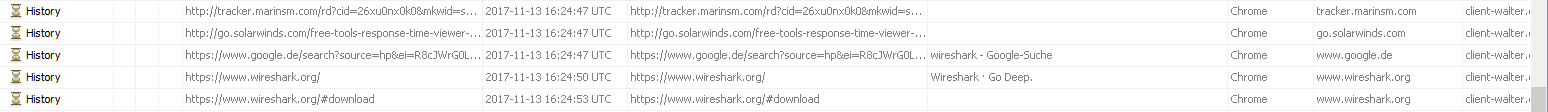
\includegraphics[width=15.8cm]{figures/wireshark_history.PNG}
	\captionof{figure}{Analyse der aufgerufenen Webseiten}
	\label{fig:wireshark_history}
\end{center}

\begin{center}
	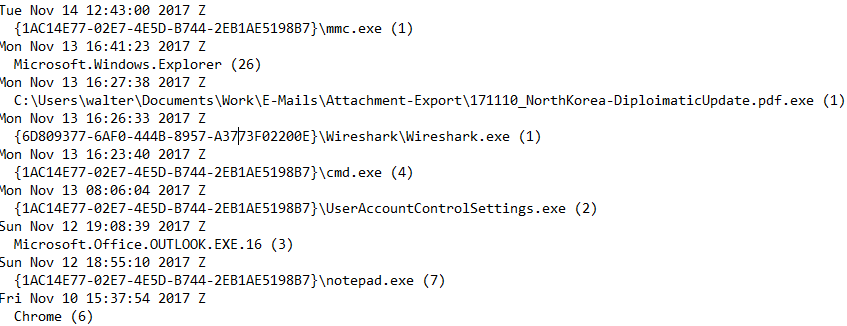
\includegraphics[width=15.8cm]{figures/wireshark_paths.png}
	\captionof{figure}{Dateipfade zu analysierten Dateien}
	\label{fig:wireshark_paths}
\end{center}

\section{Prozessliste}
Mithilfe von Volatility 2.6.1 konnten aus dem Arbeitsspeicher die aktiven und beendeten Prozesse ausgewertet werden. Dabei fiel auf, dass der verdächtige Prozess \path{171110_NorthKo} um 13.11.17 16:27 Uhr gestartet wurde und bis zur Extraktion bzw. der forensischen Sicherung des Arbeitsspeichers nicht beendet wurde. Dies bestätigt den Security Incident. Die Ausgabe von Volatility pslist ist in Abbildung X zu sehen.

Eine Minute davor um 16:26 Uhr wurde das Netzwerk Sniffing Tool Wireshark gestartet und am nächsten Tag, den 14.11.17 um 16:01 Uhr beendet. Es ist zu vermuten, dass Wireshark vom Nutzer selbst ausgeführt wurde, da es vor dem Virus gestartet wurde. Der User könnte einen verdacht gehabt haben und sicherheitshalber den Netzwerktraffic tracken wollte. Es ist zu empfehlen, den Mitarbeiter Lars Walter dazu zu befragen.
\\
\\
Es wurde in der Prozessanalyse mit Volatility der Prozess \path{171110_NorthKo} mit der Prozess-ID 6580 gefunden. Wie in Abbildung X zu sehen ist, hat diese Datei die cmd.exe Prozesse gestartet. Diese Prozesse weisen alle die bereits oben erwähnte PID 6580 der Malware als Parent-PID auf. Diese Prozesse sind verdächtig, wobei jedoch die Absicht dahinter nicht eindeutig festgestellt werden kann.

\begin{center}
	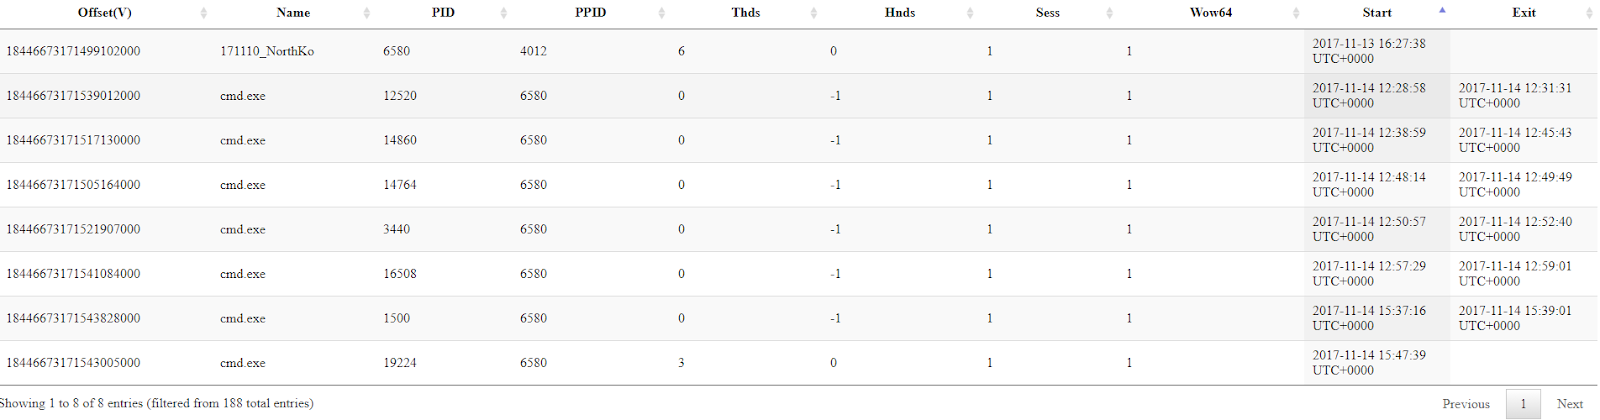
\includegraphics[width=15.8cm]{figures/processlist.png}
	\captionof{figure}{Prozessübersicht aus der Arbeitsspeicheranalyse}
	\label{fig:processlist}
\end{center}





\chapter{Weitere Aktivität des Angreifers}
Mithilfe der Timeline-Funktionalität des Forensik-Tools Autopsy wurde die verdächtig wirkende Datei fklmjsvktiq.exe wie in Abbildung \ref{fig:malware-fklm} gefunden. Diese Datei wurde am 13.11.17 um 16:53 Uhr im Dateisystem angelegt und ausgeführt.

\begin{center}
	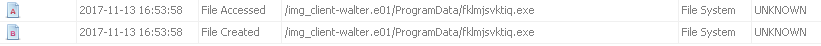
\includegraphics[width=15.8cm]{figures/malware-fklm.png}
	\captionof{figure}{Nachweis der fklmjsvktiq.exe}
	\label{fig:malware-fklm}
\end{center}

Zur weiteren Analyse wurde die Datei wie in Abbildung \ref{fig:virustotaol-fkl} auf www.virustotal.com hochgeladen.
Dabei stellte sich heraus, dass die Datei als Schadsoftware eingestuft wird. Anhand VirusTotal konnte außerdem das grobe Verhalten der Schadsoftware abgelesen werden.
\begin{center}
	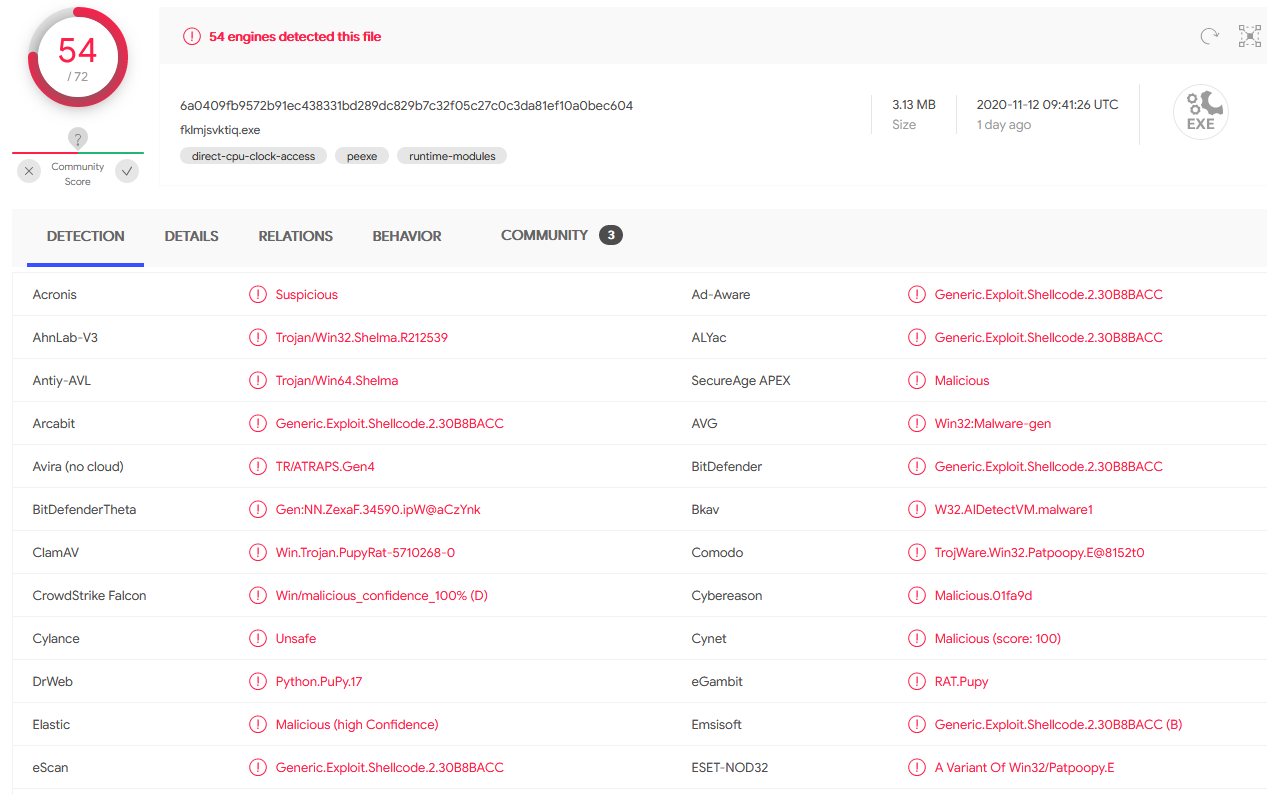
\includegraphics[width=15.8cm]{figures/virustotaol-fklm.PNG}
	\captionof{figure}{VirusTotal Auswertung zu fklmjsvktiq.exe}
	\label{fig:virustotaol-fkl}
\end{center}

Es stellte sich dabei heraus, dass die Maleware in der Lage ist, wichtige .dll Libraries wie kernel32.dll (Verwaltung von Speicher und  Ein-/Ausgabefunktionen) und user32.dll zu importieren, welche möglicherweise zu weitreichenden Eingriffen ins System genutzt wurden.
Des Weiteren werden verschiedene IP-Adressen aufgerufen wie in Abbildung \ref{fig:virustotal-fklm03} zu sehen ist, wobei die Adresse 210.122.17.27 auf einen koreanischen Server verweist und in vorliegenden Kontext daher besonders verdächtig erscheint.

\begin{center}
	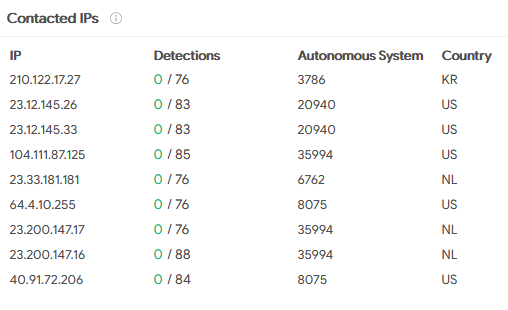
\includegraphics[width=15.8cm]{figures/virustotal-fklm03.PNG}
	\captionof{figure}{VirusTotal Analyse der aufgerufenen IP Adressen der fklmjsvktiq.exe}
	\label{fig:virustotal-fklm03}
\end{center}



\chapter{Möglicher Datendiebstahl}
Die auf VirusTotal aufgeführten IP Adressen des Viruses wie in Abbildung \ref{fig:wiresharkanalysis} zu sehen, wurden in den Wireshark Dumps analysiert. Dabei wurde eine der Verbindungen auf die IP Addresse 210.122.17.27:80 gefunden. Es fiel auf, dass sehr viele Calls auf diese IP Adresse durchgeführt wurden. Dabei wurden auch Daten übertragen, da die Calls teilweise eine sehr hohe Größe hatten.

\begin{center}
	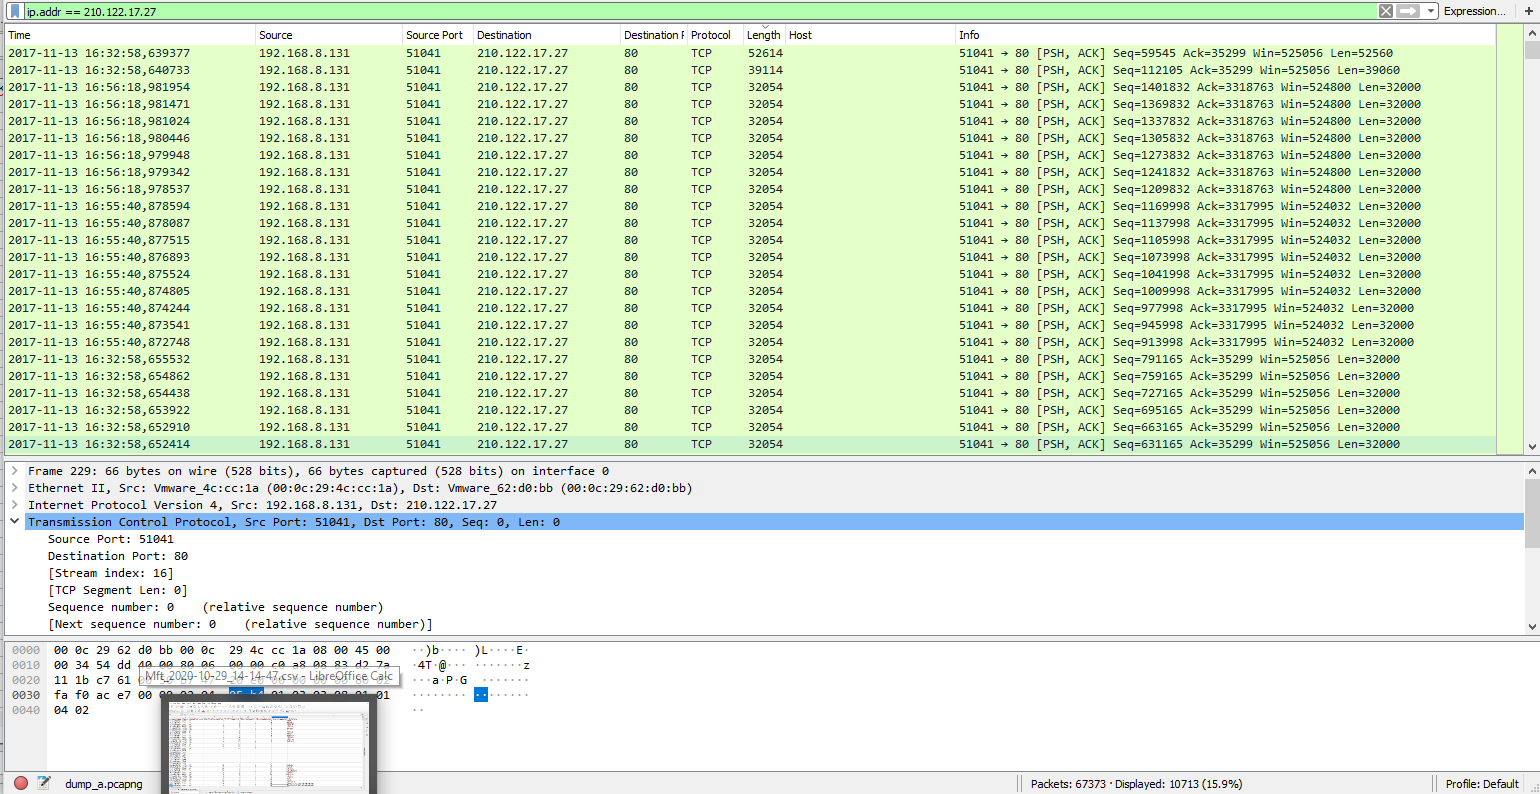
\includegraphics[width=15.8cm]{figures/wiresharkanalysis}
	\captionof{figure}{Wireshark Analyse der Calls auf 210.122.17.27:80}
	\label{fig:wiresharkanalysis}
\end{center}

In Abbildung \ref{fig:wiresharkanalysis} ist zu sehen, dass es insgesamt über 67000 Pakete mit Ziel oder Absenderadresse dieser IP Adresse hat und dass das größte Paket eine Länge von über 52000 Bytes hat. Dies deutet darauf hin, dass Daten hochgeladen wurden.

Auf \textit{who is} konnte ermittelt werden, dass sie einem asiatischen Provider zuzuordnen ist, allerdings sind durch das hohe Alter, keine genaueren Angaben möglich. Es könnte mittlerweile neu vergeben worden sein oder dieser Server war auch betroffen und wurde nur als Mittelsmann genutzt.


\begin{description}
	\item[Aufzählung] bla bla
\end{description}

\begin{enumerate}
	\item bla bla 
\end{enumerate}






\appendix

%%% Local Variables: 
%%% mode: latex
%%% TeX-master: "thesis.tex"
%%% End: 


\cleardoublepage

\footnotesize
\printindex


\end{document}
